\documentclass[12pt,a4paper]{article}
\usepackage[T1]{fontenc}     
\usepackage[utf8]{inputenc}  % Accents codés dans la fonte
\usepackage[frenchb]{babel}  % Les traductions françaises
\usepackage{numprint}        % \numprint(9,36) pour utilisation de la virgule comme séparateur décimal



\usepackage{hyperref}
\usepackage{multicol}
\setlength{\columnseprule}{1pt}


\usepackage{amsmath}         % Les maths de base

\usepackage[svgnames]{xcolor}% Pour les besoins de PythonTeX
\usepackage{geometry}        % Gestion des dimensions des pages

\usepackage{tgpagella}       % Pour changer un peu les fontes
\usepackage{tgadventor}
\usepackage{inconsolata}

%\usepackage{minted}
\usepackage{pythontex}       % Utilisation de PythonTeX

\usepackage{graphicx}        % Gestion des inclusions
\usepackage{wrapfig}

\usepackage{tikz}            % Si on veut présenter le code Python
\usepackage[framemethod=TikZ]{mdframed}
% Un environnement pour faire joli pour présenter le code Python
\newenvironment{code}{%
\begin{mdframed}[linecolor=Green,innerrightmargin=30pt,innerleftmargin=30pt,
backgroundcolor=Black!5,
skipabove=10pt,skipbelow=10pt,roundcorner=5pt,
splitbottomskip=6pt,splittopskip=12pt]
}{%
\end{mdframed}
}

% Un raccourci pour composer les unités en caractères droits
\newcommand{\U}[1]{~\mathrm{#1}}

% Présentation de l'abstract pour la problématique
\usepackage[runin]{abstract}

% Un environnement pour la problématique
\newenvironment{problematique}{
\renewcommand{\abstractname}{Problématique}
\begin{abstract}
}{
\end{abstract}
}


% Titre et auteurs du document
\title{Petit tuto \emph{git}}
\author{Charles VAN GOETHEM}
\date{}

% Et début du document proprement dit
\begin{document}

\maketitle

\begin{problematique}
Ici le but est d'apprendre à maîtriser la solution \emph{git} pour le développent de Nenufaar. L'objectif principal est de comprendre comment fonctionne \emph{git} et son utilité pour un développement collaboratif. Dans un premier temps nous allons expliquer qu'est-ce que \emph{git} puis nous prendrons un exemple concret.
\end{problematique}

\section{Première partie}

\subsection{Pourquoi j'en ai besoin ?}

Avant d'utiliser un gestionnaire de version tu te dis que tu peux très bien gérer tes versions tout seul. Tu t'organise et décide de nommé tes fichiers avec leur version respectives. Puis tu créer des archives contenant chacune des version de productions. Pour quoi apprendre à utiliser un logiciel pour faire ça ?

\begin{center}
% Inclusion d'une image: ce qui est entre crochets est un argument "optionnel", alors que l'argument obligatoire est entre accolades
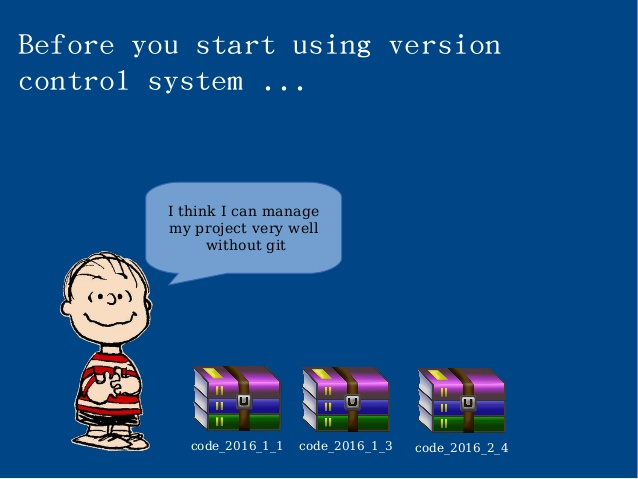
\includegraphics[width=.75\linewidth]{before_git}
\end{center}

\newpage

Puis tu continue de développer et tu crée de plus en plus de versions. C'est cool jusqu'à ce qu'un collègue arrive et nous demande la version \emph{"tu sais avec la fonction qui faisait le truc là... C'était mieux !"} et que tu recherche la bonne version...

\begin{center}
% Inclusion d'une image: ce qui est entre crochets est un argument "optionnel", alors que l'argument obligatoire est entre accolades
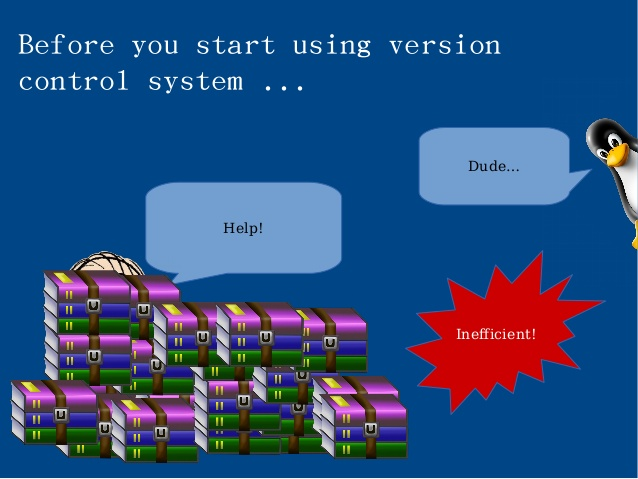
\includegraphics[width=.75\linewidth]{before_lost}
\end{center}

Maintenant tu sais pourquoi on a besoin d'un gestionnaire de version !

\subsection{\emph{git} : kézako ?}

% Inclusion d'une image: ce qui est entre crochets est un argument "optionnel", alors que l'argument obligatoire est entre accolades
\begin{wrapfigure}{r}{0.3\linewidth}
\vspace*{-1\baselineskip}

\includegraphics[width=\linewidth]{yoda_git}
\end{wrapfigure}
On s'organise un peu et on va voir le vieux sage du coin. Il nous explique alors qu'à son époque on savait coder et qu'on utilisais \emph{sccs} pour gérer les versions. Il t'explique que \emph{sccs} signifie \emph{Source Code Control System} et permet de gérer les version d'un programme ! C'est ce que tu veux mais c'est un peu vieux (1972) et puis c'est que en local... Le vieux sage t'explique alors qu'il existe des logiciels plus récent tel que \emph{subversion}, développé à la fin des années 90 et reposant sur le principe de développement centralisé, ou \emph{git}, développé au milieu des années 2000 et permettant de travailler de manière décentralisé. \emph{git} est parmi les plus répandu aujourd'hui avec plus de 12 millions d'utilisateur et en plus c'est libre !

\emph{"La route est longue mais la voie est libre..."} --- \emph{\href{https://framasoft.org/}{framasoft.org}}



\section{Seconde partie}

\begin{wrapfigure}{l}{0.3\linewidth}
\vspace*{-1\baselineskip}

\includegraphics[width=\linewidth]{git_not_simple}
\end{wrapfigure}
Utiliser \emph{git} c'est comme tout ça s'apprend ! Mais en vérité \emph{"Apprendre git, ce n'est pas si simple"} --- Boromir, fils de Denethor. On va s'intéresser ici à la théorie du système de gestionnaire de versions et aux commandes de bases de \emph{git}.

\subsection{Le gestionnaire de version}

Un gestionnaire de version de version est un outil qui va permettre d'enregistrer les évolutions d'un projet (je parle bien d'un projet pas seulement d'un programme) au cours du temps. Ainsi cela nous permettra relativement rapidement de retrouver une version antérieur du projet développé.

Ici nous nous intéressons aux systèmes de gestion de version décentralisé. En gros il existe 3 systèmes :
\begin{itemize}
\item local : très bien quand on travail seul (\emph{sccs} -- 1972) 
\item centralisé : chacun travail sur la version qu'il veut (\emph{subversion} -- 1998)
\item décentralisé : tout le monde peut disposé de toutes les versions (\emph{git} -- 2005)
\end{itemize}

\begin{center}
% Inclusion d'une image: ce qui est entre crochets est un argument "optionnel", alors que l'argument obligatoire est entre accolades
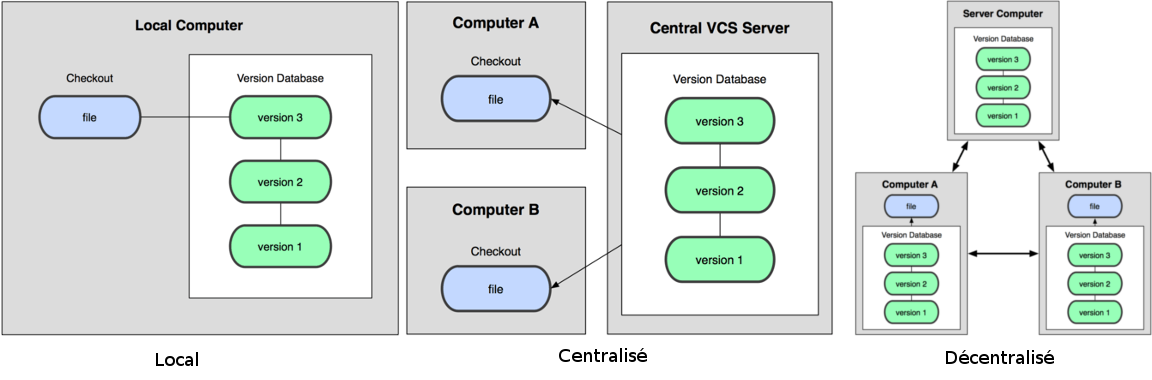
\includegraphics[width=\linewidth]{gest}
\end{center}

C'est bon ? T'es prêt pour apprendre \emph{git} ?

\newpage

\subsection{Utiliser \emph{git}}

\subsubsection{Configurer \emph{git}}

\emph{git} nécessite d'être configuré avant utilisation. Dans un premier temps on doit préciser à \emph{git} qui on est et avec quel éditeur de texte tu préfère l'utilisé :

\begin{verbatim}
$ git config --global user.name "Foo Bar"
$ git config --global user.email foo.bar@example.com
$ git config --global core.editor vim
\end{verbatim}

Là c'est cool \emph{git} c'est qui tu es et avec quel outil tu souhaite travailler. Bon on sait jamais vérifions que git sache bien qui on est :

\begin{verbatim}
$ git config user.name
Foo Bar
\end{verbatim}

On peut donc vérifier une par une les infos ou alors toutes d'un coup avec la commande suivante :

\begin{verbatim}
$ git config --list
user.name=Foo Bar
user.email=foo.bar@example.com
color.diff=auto
color.status=auto
color.branch=auto
push.default=matching
core.editor=vim
\end{verbatim}

\subsubsection{Initialiser un projet}

Bon maintenant on va voir comment créer un nouveau projet. Sans git c'est facile on crée un nouveau répertoire :

\begin{verbatim}
$ mkdir Unicorn_project
\end{verbatim}

Et avec \emph{git} pas d'affolement c'est très simple aussi. On utilise \emph{git} pour initialiser notre projet :

\begin{verbatim}
$ git init Unicorn_project
\end{verbatim}

Félicitation dans les deux cas vous avez créé votre premier projet ! Par contre on est en droit de se poser la question : \emph{Pourquoi diable faire comme ça ?}

Et bien en utilisant la commande \emph{git init} on crée également le répertoire \emph{.git}. Ce répertoire contient toute les infos dont git a besoin pour gérer les versions.

\subsubsection{Travailler}

C'est bien beau tout ça mais il faut travailler maintenant. Pour apprendre les bases de \emph{git} on va supposer que l'on travail seul.

Alors imaginons que l'on crée un super code :
\begin{verbatim}
$ vi my_awesome_script.pl
$ more my_awesome_script.pl
#/usr/bin/perl

print "My little pony !\n";
\end{verbatim}

Voilà notre premier script du projet finit ! On peut utiliser la commande suivante pour voir l'avancement du projet.

\begin{verbatim}
Sur la branche master

Validation initiale

Fichiers non suivis:
  (utilisez "git add <fichier>..." pour inclure dans ce qui sera
validé)

	my_awesome_script.pl

aucune modification ajoutée à la validation mais des fichiers non
suivis sont présents (utilisez "git add" pour les suivre)
\end{verbatim}

Là \emph{git} nous signale que l'on a un fichier qui n'est pas \emph{"suivi"}. Cela signifie que ce fichier n'est pas encore traité par \emph{git}. Pour lui signaler que l'on veux le traiter on l'ajoute (on verra plus tard comment ignorer certains fichiers), et on vérifie :

\begin{verbatim}
$ git add my_awesome_script.pl 
$ git status
Sur la branche master

Validation initiale

Modifications qui seront validées :
  (utilisez "git rm --cached <fichier>..." pour désindexer)

	nouveau fichier: my_awesome_script.pl
\end{verbatim}

Bon et maintenant il faut \emph{"commiter"} ses actions. \emph{"Commiter"} son code signifie soumettre, archiver son code. En même temps que l'on \emph{commit} le code on doit ajouter un message qui définit la modification effectuer. Traditionnellement le message "Initial commit" est associé au premier \emph{commit}.

\begin{verbatim}
$ git commit -m "Initial commit"
[master (commit racine) e023001] Initial commit
 1 file changed, 3 insertions(+)
 create mode 100644 my_awesome_script.pl
$ git status
Sur la branche master
rien à valider, la copie de travail est propre
\end{verbatim}

Bon ben déjà avec ces quelques commandes on peut archiver nos projets de façon propre. C'est pas mal pour un début !


\subsubsection{Ignorer des fichiers}

\begin{wrapfigure}{l}{0.3\linewidth}
\vspace*{-1\baselineskip}

\includegraphics[width=\linewidth]{dontcare}
\end{wrapfigure}

Bon alors c'est déjà pas mal ! Maintenant on va apprendre a ignorer des fichiers. En effet, dans un grand nombre de projets on génère des fichiers qu'il n'est pas utile d'archiver (notamment des fichiers temporaires, des logs...).

C'est pourquoi on peut indiquer à \emph{git} que certains de nos fichiers ne sont pas à prendre en compte. Ici on va voir deux exemple : une répertoire contenant les logs et des fichiers \emph{.bak} généré par un éditeur.

\begin{verbatim}
$ git status
Sur la branche master
Fichiers non suivis:
  (utilisez "git add <fichier>..." pour inclure dans ce qui sera
validé)

	PinkUnicornOfLove.sh
	PinkUnicornOfLove.sh.bak
	log/

aucune modification ajoutée à la validation mais des fichiers non
suivis sont présents (utilisez "git add" pour les suivre)
\end{verbatim}

On a ici un script (\emph{PinkUnicornOfLove.sh}),  un fichier temporaire (\emph{PinkUnicornOfLove.sh.bak}) et un répertoire de log. Pour ignorer ces fichiers et répertoires on va créer un fichier spécial :

\begin{verbatim}
$ vi .gitignore
$ more .gitignore 
*.bak
log/
$ gits
Sur la branche master
Fichiers non suivis:
  (utilisez "git add <fichier>..." pour inclure dans ce qui sera
validé)

	.gitignore
	PinkUnicornOfLove.sh

aucune modification ajoutée à la validation mais des fichiers non
suivis sont présents (utilisez "git add" pour les suivre)
\end{verbatim}

\begin{minipage}{0.25\linewidth}
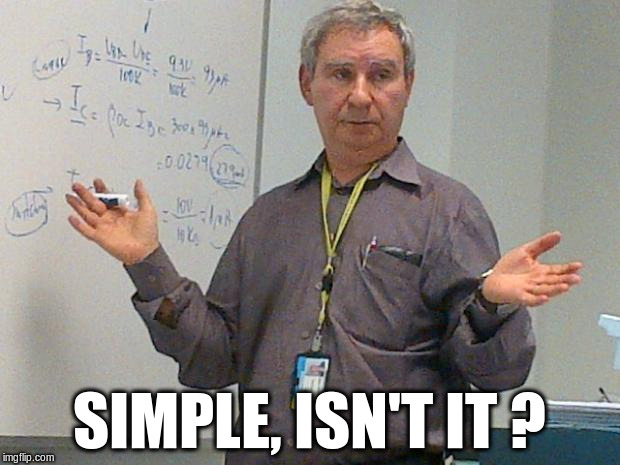
\includegraphics[width=\linewidth]{simple}
\end{minipage}\hfill
\begin{minipage}{0.7\linewidth}
On voit qu'une fois le fichier \emph{.gitignore} créé le fichier \emph{.bak} et le répertoire \emph{log} ne sont plus sur la liste des fichiers non-suivis.

Et voilà on sait maintenant utiliser \emph{git}. Au moins pour gérer de petits projets.
\end{minipage}

\subsection{Travailler à plusieurs}

Maintenant on va compliquer un peu les choses avec le travail à plusieurs, mais en vérité c'est pas beaucoup plus complexe (en tout cas pour le début).

\subsubsection{cloner un dépôt}

Dans un premier temps on va apprendre a cloner un dépôt déjà existant. Cela veut dire que l'on va créer une copie exacte du premier projet. Les deux copies auront donc le même historique et sont donc toute les deux autant légitime l'une que l'autre.

\begin{verbatim}
$ git clone Path/project_A Path/project_b
Clonage dans 'project_b'...
remote: Counting objects: 14, done.
remote: Compressing objects: 100% (11/11), done.
remote: Total 14 (delta 5), reused 0 (delta 0)
Réception d'objets: 100% (14/14), 5.09 KiB | 0 bytes/s, fait.
Résolution des deltas: 100% (5/5), fait.
Vérification de la connectivité... fait.
\end{verbatim}

\subsubsection{Maintenir à jour sa copie}

On va partir de l'hypothèse que le dépôt \emph{project\_A} est la référence et que le dépôt \emph{project\_b} est la copie locale. On suppose que des modifications sont apportés au dépôt A sans que vous ayez modifié le dépôt B.

Lorsque vous ferais un \emph{git status} dans le dépôt B vous ne verrais pas de modification. En effet il est à jours avec lui-même, il faut tester si le dépôt B est à jours avec le dépôt A.

\begin{verbatim}
$ git status
Sur la branche master
Votre branche est à jour avec 'origin/master'.
rien à valider, la copie de travail est propre
$ git remote update
Récupération de origin
remote: Counting objects: 3, done.
remote: Compressing objects: 100% (3/3), done.
remote: Total 3 (delta 1), reused 1 (delta 0), pack-reused 0
Dépaquetage des objets: 100% (3/3), fait.
Depuis Path/project_A
   69e3c98..1bb5353  master     -> origin/master
$ git status
Sur la branche master
Votre branche est en retard sur 'origin/master' de 1 commit, et peut
être mise à jour en avance rapide.
  (utilisez "git pull" pour mettre à jour votre branche locale)
rien à valider, la copie de travail est propre
\end{verbatim}

\emph{git} nous signale que nous ne sommes plus à jours par rapport au dépôt A. Il nous précise de faire un \emph{git pull}. Cette commande permet de récupérer les modifications sur le dépôt A.

\begin{verbatim}
$ git pull
Mise à jour 69e3c98..1bb5353
Fast-forward
 README.md | 2 +-
 1 file changed, 1 insertion(+), 1 deletion(-)
\end{verbatim}

On voit que l'on a récupéré deux modification sur le fichier README.md.

\subsubsection{Envoyer ses modifications}

Maintenant que l'on sait maintenir à jour un dépôt, on va voir comment envoyer ses modifications. Là aussi c'est simple une commande permet de le faire :

\begin{verbatim}
$ vim README.md 
$ git commit -m "little"
[master 26074e3] little
 1 file changed, 1 insertion(+), 1 deletion(-)
$ git push
Décompte des objets: 3, fait.
Delta compression using up to 8 threads.
Compression des objets: 100% (3/3), fait.
Écriture des objets: 100% (3/3), 364 bytes | 0 bytes/s, fait.
Total 3 (delta 1), reused 0 (delta 0)
remote: Resolving deltas: 100% (1/1), completed with 1 local objects.
To https://github.com/...../
   1bb5353..26074e3  master -> master
\end{verbatim}

Et voilà la modification est envoyée ! C'est ultra-simple non ? Bon alors évidemment là on suppose que l'on a bien fait un pull juste avant de modifier notre programme et que personne ne l'a modifié au même endroit...

\subsubsection{La théorie des branches}

\begin{minipage}{0.7\linewidth}
Les branches sont très importante sous \emph{git}. On verra dans la section suivante avec un exemple concret sur Nenufaar comment on pourra les utiliser.
\end{minipage}\hfill
\begin{minipage}{0.25\linewidth}

\includegraphics[width=\linewidth]{branch}
\end{minipage}

Pour faire simple les branches sont des variations de la branche principale, dite \emph{"master"}. On vas notamment souvent trouver une branche stable qui servira au versions des projets, la branche de production (\emph{master}), et une seconde branche qui servira a stocker les avancer régulière entre deux points stable, la branche de développement. Mais on va également pouvoir avoir un ensemble d'autres branches qui seront des corrections de bugs par exemple.

\centerline{
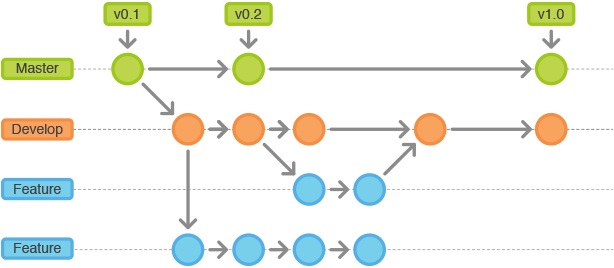
\includegraphics[width=0.7\linewidth]{git-branch}}

Sur ce graphique on voit 3 points stable de version (en vert) sur la branche \emph{master}. Ensuite on trouve une branche de développement (en orange), puis des branches concernant les features, ajout de nouvelles fonctions au programme (en bleu). La philosophie des auteurs, pour ce cas, est :
\begin{itemize}
\item[$\bullet$] pas de commit sur les branches \emph{master} et \emph{dev} ;
\item[$\bullet$] une branche par feature ;
\item[$\bullet$] les \emph{features} sont fusionnées sur la branche \emph{dev}.
\end{itemize}

Je vais pas aller beaucoup plus loin sur les branches puisque je l'expliquerais à l'aide d'un exemple concret plus tard. Je vais quand même expliquer les quelques commandes utiles pour leur manipulation.

Les commande suivantes servent à créer, rejoindre, fusionner et supprimer des branches.

\begin{verbatim}
$ git branch MyBranch		### créer la branche MyBranch
$ git checkout MyBranch		### rejoindre la branche Mybranch
$ git checkout -b MyBranch	### créer et rejoindre la branche Mybranch
$ git merge MyBranch		### fusionner la branch MyBranch avec la
branche courante
$ git branch -d Mybranch	### supprimer la branche MyBranch
\end{verbatim}


% \subsubsection{Travailler sur \emph{bitbucket}}

% Maintenant on va compliquer un peu les choses avec le travail à plusieurs. Ici on va voir l'application sur \emph{bitbucket}. \emph{Bitbucket} est un service d'hébergement et de gestion de développement logiciel.

% \paragraph{Créer son compte} Aller sur \emph{\href{https://bitbucket.org}{https://bitbucket.org}}

% %\subsubsubsection{Relier son compte de façon sécurisé}





% \section{Seconde partie}

% \subsection{Expérience}

% \subsection{Observations}

% \subsection{Conclusion}

% \section{Conclusion générale du TP}
% http://www.slideshare.net/shengwen1997/brief-tutorial-on-git

\end{document}